\subsection{MVC Framework}
\label{sec:mvc}
The Model-View-Controller (MVC) was originally designed by Trygve M. H. Reenskaug in 1979, who was at that time working for Xerox PARC. The goal was to create an environment in which the users (developer, customer etc.) could preserve the original perception of the data structure, while being able to view and edit portions of it. \cite{mvcxeroxparc}

\subsubsection{Components}

The MVC framework consists of three different types of components; Views, controllers and models. Each created with a different purpose, see figure \ref{fig:mvc-drawing}

\begin{figure}[htb]
	\centering
		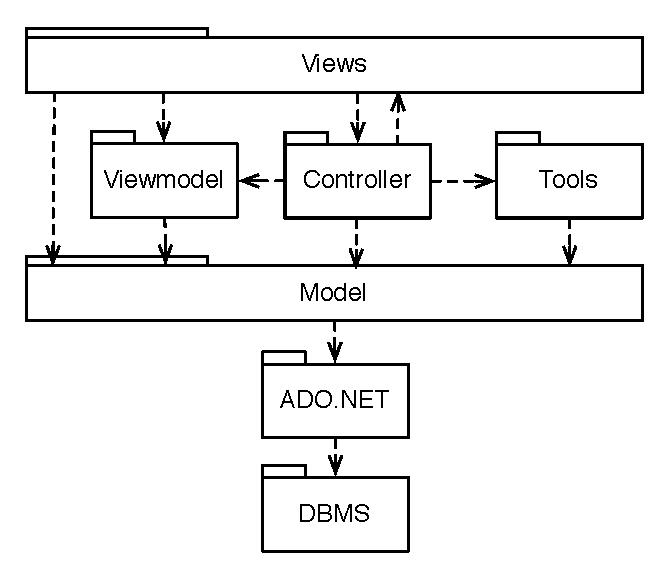
\includegraphics[width=0.90\textwidth]{input/implementation/mvc/mvc.pdf}
	\morscaption{These are the three main components in the MVC}
	\label{fig:mvc-drawing}
\end{figure}



\paragraph{Models}
The models are the components that handle the data domain of the application, it is typically mapped to a database from which it reads and writes data. This way developers can handle the data, without worrying about the actual data connection.

\paragraph{Views}
The views display the data and UI. They are typically created with data provided from the model. These views are full-featured (X)HTML, with the addition of C\# or Visual Basic code, to fetch content from the model.

\paragraph{Controllers}
The controllers reacts to user requests the users provides through the UI. Based on this they decide which view should be rendered. If the data the view should display does not exist in the model (input, etc.) the controller can also provide this data to the view to display.

\paragraph{Master-page}
Master-pages is not a part of MVC as a design-idea, it is a component implemented by Microsoft. The master-page is a page that is always loaded when displaying a view. Like the view, it consists of (X)HTML and C\#/ Visual Basic, however, it also has content-containers. These containers can be created anywhere on the web page, and are filled with content by views.

\paragraph{Structure}
An interesting thing about MVC is that there are no actual HTML files, all content is generated generically as the users interacts with the different components within the web page. When entering an URL the user actually call methods in controllers, the user can even add parameters to the calls. The controllers then redirects the user to the correct view based on the input and the method called. The view then executes, which results in a plain web page that can be displayed in a browser.

Because of the separation into three independent modules, developers are able to create different parts of the application with different kind of approaches, thus enabling them to better manage complexity, create applications with a high maintainability, and create UI that does not have to show the actual data structure.

%\subsubsection{Data validation}
%Client side validation
%Server Side validation

\paragraph{Testing}
When creating web applications with MVC you have the possibility of creating unit tests to thoroughly test your code. These tests can be automatically generated from within Visual Studio, and run as a separate function, in order to allow the developer to test for all possible inputs. For a more detailed description of Unit-testing in MVC, look in the section \ref{chap:testing}. \cite{mvcconcept, aspdotnet}